\section{Frequenzverhalten}

Da jede leitende Fläche eine Kapazität gegenüber der umliegenden Flächen besitzt, müssen zur Einschätzung des Frequenzgangs diverse Kapazitäten berücksichtigt werden.


\subsection{Parasitäre Kapazitäten in MOS-Transistoren}

An einem FET können grundsätzlich an jedem Knoten parasitäre Kapazitäten auftreten.
Für die meisten Betrachtungen sind jedoch nicht alle davon relevant. 

\smallskip

\textbf{Achtung:} Die gezeigte Kleinsignalersatzschaltung des Transistors gilt für $V_{\rm SB} = \qty{0}{\volt}$


\begin{minipage}[t]{0.26\columnwidth}
    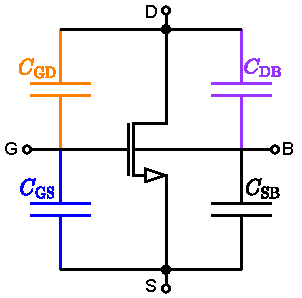
\includegraphics[width=\columnwidth, align=t]{images/08_parasitaere_C_am_FET.pdf}
\end{minipage}
\hfill
\begin{minipage}[t]{0.6\columnwidth}
    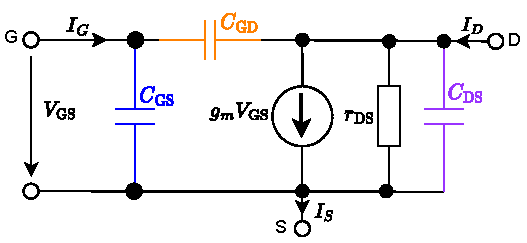
\includegraphics[width=\columnwidth, align=t]{images/08_MOSFET_parasitaere_kapazitaeten_ersatzschaltung.pdf}
\end{minipage}


\subsubsection{Parasitäre Kapazitäten in der Praxis}
\label{Parasitäre Kapazitäten in der Praxis}

In der Praxis gilt typischerweise:

\smallskip

\begin{outline}
    \1 Die domnierende Kapazität ist $\cbl{ C_{\rm GS} }$
    \1 Falls kein Body-Effekt auftritt bzw. $V_{\rm SB} = \qty{0}{\volt}$ ist, gilt Folgendes:
        \2 $C_{\rm SB}$ ist kurzgeschlossen und somit wirkungslos
        \2 $\cvt{ C_{\rm DB} = C_{\rm DS} }$ (wie in gezeigter Kleinsignalersatzschaltung)
    \1 $\cor{ C_{\rm GD} }$ ist vom \textbf{Miller-Effekt} betroffen, falls der Transistor eine Spannungsverstärkung hat
\end{outline}


\paragraph{Typische Werte für parasitäre Kapazitäten ($W = L = \qty{5}{\micro \meter}$)}

\resizebox{\columnwidth}{!}{
    \begin{tabular}{lllll}
    \hline
    \textbf{Arbeitsbereich} & $\bm{C_{\rm GS}}$                 & $\bm{C_{\rm GD}}$                 & $\bm{C_{\rm SB}}$                 & $\bm{C_{\rm DB}}$                 \\
    \hline  
    \textbf{Gesättigt}      & $C_{\rm GS0t} + 2/3 C_{\rm oxt}$  & $C_{\rm GD0t}$                    & $C_{\rm jSBt} + 2/3 C_{\rm BCt}$  & $C_{\rm jDBt}$                    \\
    \textbf{Typ. Wert}      & $\qty{103}{\femto \farad}$        & $\qty{0.0555}{\femto \farad}$     & $\qty{14.9}{\femto \farad}$       & $\qty{1.7}{\femto \farad}$        \\
    \hline
    \textbf{Ungesättigt}    & $C_{\rm GS0t} + 1/2 C_{\rm oxt}$  & $C_{\rm GD0t} + 1/2 C_{\rm oxt}$  & $C_{\rm jSBt} + 1/2 C_{\rm BCt}$  & $C_{\rm jDBt} + 1/2 C_{\rm BCt}$  \\
    \textbf{Typ. Wert}      & $\qty{77.555}{\femto \farad}$     & $\qty{77.555}{\femto \farad}$     & $\qty{11.6}{\femto \farad}$       & $\qty{11.6}{\femto \farad}$       \\
    \hline
    \end{tabular}
}

\medskip

\textbf{Hinweis:} Die Kapazitäten in den Formeln sind Technologie-Parameter.

\smallskip

\begin{tabular}{ll}
    $C_{\rm oxt}$                                   & Nutzkapazität                                     \\
    $C_{\rm GDt}$ / $C_{\rm GSt}$                   & Parasitäre Kapazitäten verursacht durch Overlap   \\
    $C_{\rm jSBt}$ / $C_{\rm jDSt}$ $C_{\rm jBCt}$  & Parasitäre Kapazitäten wegen Raumladungszone      \\
\end{tabular}


% \subsubsection{Nutzkapazität}
% \[
%     C_{oxt} = C_{\rm ox} \cdot W_{eff} \cdot L_{eff}
% \]

% \subsubsection{Parasitäre Kapazitäten}
% Gate-Drain- und Gate-Source-Kapazitäten durch Overlap
% \[
%     C_{GDt} = C_{GD} \cdot W_{eff} \cdot L_{eff}
%     \qquad
%     C_{GSt} = C_{GS} \cdot W_{eff} \cdot L_{eff}
% \]

% Source-Bulk- und Drain-Bulk-Kapazitäten durch Raumladungszone
% \[
%     C_{jSBt} = C_{jSB} \cdot A_S + C_{jswSB} \cdot P_S
%     \qquad
%     C_{jDSt} = C_{jGS} \cdot A_S + C_{jswDB} \cdot P_D
% \]
% $C_{jsw}$: Side Wall Kapazität
% $P$: Perimiter

% Kanal-Bulk-Kapazität durch Raumladungszone
% \[
%     C_{jBCt} = C_{jBC} \cdot W_{eff} \cdot L_{eff}
% \]

% Junction-Bulk-Kapazität
% \[
%     C_{jBC}
% \]



\subsection{Miller-Approximation / Miller-Effekt}

Die (parasitäre) Kapazität zwischen Eingang und Ausgang (typischerweise $C_{\rm GD} = C_m$) der Schaltung wird durch die Verstärkung des Transistors stark vergrössert.
Die Miller-Approximation bekommt diese 'Problematik' für Abschätzungen von Hand in den Griff.

\begin{center}
    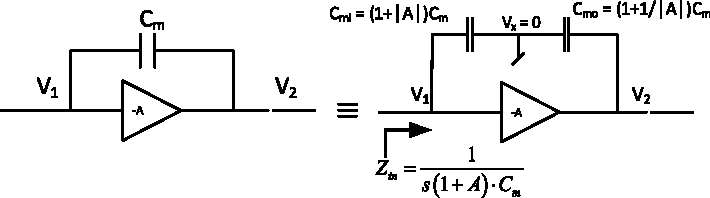
\includegraphics[width=0.85\columnwidth]{images/08_Miller_C.pdf}
\end{center}


Das Miller Theorem postuliert, dass die linke Schaltung durch Wählen von $Y_1$ und $Y_2$ als 

\vspace{-0.2cm}

\[
    Y_1(s) = Y(s) (1+A) \qquad \text{und} \qquad Y_2(s) = Y(s) \left( 1+\frac{1}{A} \right)
\]

\vspace{-0.1cm}

äquivalent gemacht werden können.
Es kann durch einfaches Einsetzen bewiesen werden.


\subsubsection{Einfluss der Miller-Kapazität}

Die Miller-Kapazität $C_m$ erscheint 

\smallskip

\begin{minipage}[t]{0.6\columnwidth}
    \begin{itemize}
        \item multipliziert mit $1+\abs{A}$ am Eingang als $C_{\rm mi}$ und
        \item multipliziert mit $1+\abs{\frac{1}{A}}$ am Ausgang als $C_{\rm mo}$.
    \end{itemize}
\end{minipage}
\hfill
\begin{minipage}[t]{0.33\columnwidth}
    $\abs{A}$ entspricht dem DC-Gain des Transistors
\end{minipage}



\subsubsection{Nachteile der Miller-Approximation}
 
\begin{itemize}
    \item Durch Verschieben des Miller-C aus dem Vorwärtspfad stimmt die UTF nach Ersetzen des $C_m$ nicht mehr.
    \item Das Miller-Theorem geht von konstantem Frequenzgang der Verstärkung aus. Es stimmt folglich nur für die tieferen Frequenzen.
\end{itemize}


\subsubsection{Brauchbarkeit der Miller-Approximation}

Mit der Miller-Approximation kann die Übertragungsfunktion (aus der Kleinsignalersatzschaltung) berechnet werden.
Man erhält eine genaue Formel, aus welcher die Polfrequenzen ermittelt werden könne.
In diese genauen Formeln werden dann \textbf{approximative / ungenaue Werte} eingesetzt.

\smallskip

\textbf{ \textrightarrow\ Miller-Approximation in Praxis nicht brauchbar! \textrightarrow\ Simulation! }



\subsection{Frequenzverhalten durch Zero Value Time Constant Analysis}

Die Zero Value Time Constant Analysis ist eine Methode, um die \textbf{Bandbreite} einer Schaltung abzuschätzen und zu bestimmen, welche Knoten für das Frequenzverhalten am wichtigsten sind \textrightarrow\ \textbf{dominante Pole}


\subsubsection{Vorgehen -- Zero Value Time Constant Analysis}

{
\setlist[enumerate, 1]{label=\bfseries\arabic*.}
\setlist[enumerate, 2]{label=\bfseries\alph*)}
\renewcommand{\outlinei}{enumerate}
\renewcommand{\outlineii}{enumerate}
\begin{outline}
    \1 Kleinsignalersatzschaltung erstellen
    \1 Für alle $C_k$ die zugehörige \textbf{Zeitkonstanten} bestimmen:
        \2 Alle übrigen $C_{i \neq k} = 0$ setzen
        \2 Betrachtetes $C_k$ durch eine Spannungsquelle ersetzen und den von $C_k$ her gesehenen Kleinsignalwiderstand bestimmen
        \2 Zeitkonstante $\tau_k$ und Polfrequenz $f_{\rm pk}$ für betrachtetes $C_k$ berechnen
    \1 Approximiertern Frequenzgang aus DC-Verstärkung und gefundenen Polstellen \\
        (bei $f_{\rm pk}$) zusammensetzen und bei Bedarf in Bode-Diagramm einzeichnen
\end{outline}
}

$$ \tau_k = R_k C_k \qquad \qquad f_{pk} = \frac{1}{2 \pi \tau_k} $$

\textbf{ \textrightarrow\ Der dominante Pol ist derjenige mit dem grössten $\bm{\tau_k}$}


\subsubsection{Interpretation der Polstellen}

\begin{minipage}[t]{0.48\columnwidth}
    \paragraph{Bandbreite (GBP)}

    Wird durch den \textbf{ersten Pol} bestimmt

    \vspace{-0.2cm}

    $$ \text{GPB} \approx f_{\rm p1} \cdot A_{\rm DC} $$
\end{minipage}
\hfill
\begin{minipage}[t]{0.48\columnwidth}
    \paragraph{Stabilität}

    Wird durch den \textbf{zweiten Pol} bestimmt

    \vspace{-0.2cm}

    $$ f_{180^\circ} \approx f_{\rm p2} $$
\end{minipage}


\subsubsection{Typische Werte für parasitäre Komponenten}

\begin{outline}
    \1 Typische Werte für parasitäre Kapazitäten: siehe Abschnitt \ref{Parasitäre Kapazitäten in der Praxis}
    \1 Typische Werte für Kleinsignalwiderstände (Innenwiderstände) an Transistor-Knoten gemäss folgender Tabelle
\end{outline}


\renewcommand{\arraystretch}{1.2}
\begin{ctabular}{lccc}
                    & \textbf{Innenwiderstand}      & \textbf{hoch / tief}  & \textbf{typisch}      \\
    \textbf{Gate}   & $r_{\rm iG}$                  & unendlich             & \qty{}{\giga \ohm}    \\
    \textbf{Drain}  & $r_{\rm  DS} = \frac{1}{g_o}$ & hoch                  & \qty{}{\mega \ohm}    \\
    \textbf{Source} & $\frac{1}{g_m}$               & tief                  & \qty{}{\kilo \ohm}    \\
\end{ctabular}
\renewcommand{\arraystretch}{1}

\begin{outline}
    \1 Vorsicht bei $C_{GD}$: Sollte der Transistor eine Spannungsverstärkung haben, so muss der Miller-Effekt berücksichtigt werden.
    \1 Weiter ist $C_{GD}$ bei hohen Frequenzen oft als erstes kurzgeschlossen, für den zweiten Pol muss dieser als kurzgeschlossen betrachtet werden.
\end{outline}

